The trend of both curiosity and profit-driven human development has caused a
surge in the amount of openly accessible raw data. More often than not, the data is generated much faster than it can be processed into something interpretable or useful. In the endeavor of keeping up with the inflow of information, there are two major factors that significantly hinder our progress. First, Moore’s law implicitly sets a physical limit to the number of transistors that can be placed on a chip, consequently limiting how powerful and how fast electronic systems can become (barring a paradigm shift in the fundamental design of semiconductors). The second is the Nyquist-Shannon sampling theorem (NST), which limits the range of frequencies a recording device can successfully capture. This states that given that you know a signal's highest frequency component $f_B$, sampling it at a rate $f_S$ that is at least twice this frequency is sufficient to capture all of the pertinent information regarding that signal: that is $f_S \geq 2f_B$, where $f_B$ is known as the Nyquist rate \cite{Shannon1949}, and also as the signal bandwidth. For signals that are not naturally bandlimited, such as images, the ability reproduce a signal is dependent on the device's resolution and still follows the same principle: there should be at least twice the number of pixels codimensional with the image's highest spatial frequency. For practical day-to-day use, the NST will suffice. However, issues arise when bandwidth and storage are at a premium. Typically, after sensing a signal, not all of the raw data is stored. Rather, this data is converted to a compressed format by systematically discarding values such that the loss of information is virtually imperceptible. Thus, the process of acquiring massive amounts of data followed by compression is extremely wasteful. CS aims to directly acquire the parts of the signal that would otherwise survive this compression stage in the classical sampling scheme.

Consider a signal $\vec{x} \in \mathbb{R}^{n}$; this notation indicates that $\vec{x}$ is a vector of cardinality $n$, containing elements over the field of real numbers ($\vec{x}$ can also easily be a complex vector, but for the purposes of this chapter, it is sufficient to emphasize that we are working with real-valued signals). The process of acquisition or sensing this signal can be modeled as a linear system, where the physical signal properties we wish to capture are transformed into digital values by applying a linear transformation

\begin{equation}\label{eq:cesa-linear}
	\vec{y} = \vec{A} \vec{x}
\end{equation}

\noindent or in the literature of signal processing \cite{Candes2008b}, by correlating them with a waveform basis

\begin{equation}\label{eq:cesa-correlation}
	y_k = \innerproduct{\vec{x}}{\vec{a}_k} , \quad k \in \mathbb{N} \leq n
\end{equation}

In conventional sampling, $\vec{a}_k$ are Dirac basis vectors which turn $\vec{y}$ into a vector containing samples of $\vec{x}$ in the temporal or spatial domain; if $\vec{a}_k$ are Fourier basis vectors (i.e., sinusoids), then $\vec{y}$ is a vector of Fourier coefficients. If the signal has been sampled sufficiently in the sense that the number of measurements $m$ is equal to the dimension $n$ of the signal, then $\vec{A}$ is a square matrix, and the original signal $\vec{x}$ can be reconstructed from the information vector $\vec{y}$ by inversion of \eqref{eq:cesa-linear}. However, the process of recovering $\vec{x} \in \mathbb{R}^n$ from $\vec{y} \in \mathbb{R}^m$ becomes ill-posed when we consider the undersampled case ($m \ll n$), as the sensing matrix $\vec{A} \in \mathbb{R}^{m \times n}$---whose row vectors are denoted as $\vec{a}_m$---causes the system to become underdetermined: there exist infinitely many candidate solutions $\bm\hat{\vec{x}}$ which satisfy \eqref{eq:cesa-linear}. To add to this, we also consider the possibility that the measurements are not perfect, and are contaminated with noise. How then do we recover a signal from measurements which are incomplete and most likely inaccurate? The answer lies in enforcing constraints based on models of natural signals, as well as constraints based on optimization techniques.

\section{Sparsity}
\label{sec:sparsity}

Most natural signals, especially those with some underlying periodicity, can be represented sparsely when expressed in the appropriate basis. This process of ``sparsifying'' can be expressed as

\begin{equation}\label{eq:sparsify}
	f = \innerproduct{\vec{x}}{\bm\psi(k)}
\end{equation}

Similar to \eqref{eq:cesa-correlation}, this involves correlating the signal with the appropriate basis function to yield a representation in the sparse domain. Image information, for example, are commonly expressed in the DCT domain by

\begin{equation}\label{eq:dct}
	f_k = \sum_{n=0}^{N-1} x_n \cos\qty[\frac{\pi}{N}\qty(n + \frac{1}{2})k] , \quad 0 \leq k < N
\end{equation}

\noindent and its corresponding inverse is

\begin{equation}\label{eq:idct}
	x_k = \frac{1}{2}f_0 + \sum_{n=1}^{N-1} f_n \cos\qty[\frac{\pi}{N} \qty(k + \frac{1}{2})n] , \quad 0 \leq k < N
\end{equation}

\noindent where the cosine term corresponds to $\bm\psi(k)$ in \eqref{eq:sparsify}. We can express \eqref{eq:dct} more conveniently as $\vec{f} = \bm\Psi \vec{x}$, where $\bm\Psi \in \mathbb{R}^{n \times n}$ is the sparsifying matrix. Figure \ref{fig:sparsity} shows this sparsifying process in action: given a test image, taking its Daubechies 8 discrete wavelet transform (D8 DWT) and zooming into a random subset shows that most of the signal energy is concentrated in just a few of the coefficients. All the other coefficients, when compared to the $k$ highest coefficients, are practically zero; such a signal is referred to as $k$-sparse. The compressed image resulting from discarding all but the 25,000 highest coefficients and performing the inverse transform shows that any difference from the original image is virtually imperceptible. A similar concept is used in JPEG compression, wherein an image is divided into $8 \times 8$ blocks, and in each block, a certain number of DCT coefficients are discarded depending on the desired quality factor $Q$ \cite{itu-jpeg}.

\begin{figure}[htb]
	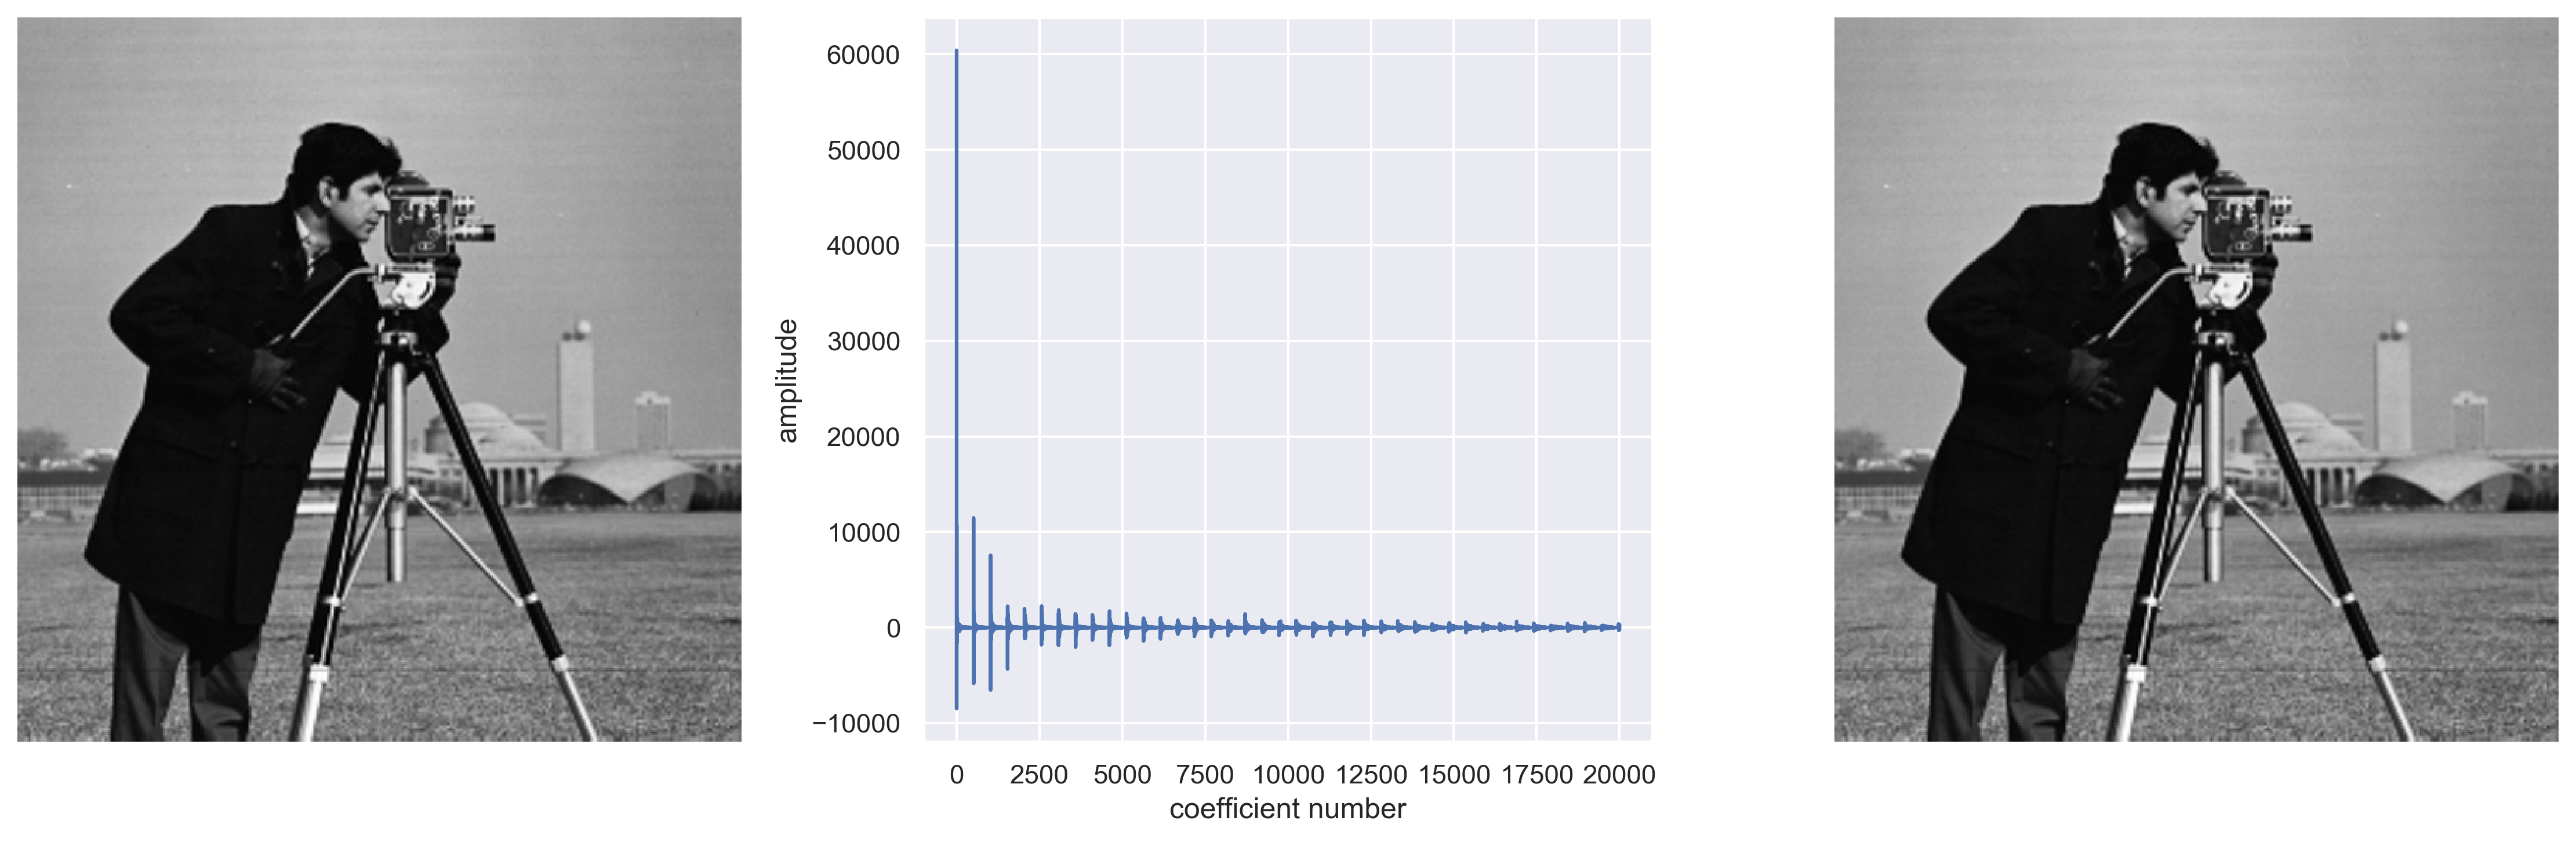
\includegraphics[width=\textwidth]{C2-sparsity.png}
	\caption{Original $512 \times 512$, 8-bit image (left), and a random subset (for better visibility) of its D8 DWT coefficients (middle). Most of the signal energy is concentrated in just a few terms. By discarding all but the 25,000 highest coefficients and performing the inverse transform, the resulting image (right) is perceptually no different from the original.}
	\label{fig:sparsity}
\end{figure}


\section{Incoherence}
\label{sec:incoherence}

Suppose we have two matrices $\bm\Phi$ and $\bm\Psi$ which are involved in the sensing of a signal. As before, $\bm\Psi$ is the sparsifying matrix which converts the signal into a sparse representation, and $\bm\Phi$ is the actual sensing matrix. The coherence between these two bases is expressed as

\begin{equation}\label{eq:coherence}
	\mu\qty(\bm\Phi, \bm\Psi) = \sqrt{n} \max_{0 \leq i,j < n} \abs{\innerproduct{\bm\varphi_i}{\bm\psi_j}}
\end{equation}

In other words, the coherence is the measure of the largest correlation between the column vectors of $\bm\Phi$ and $\bm\Psi$. In compressive sensing, we are interested in low-coherence basis pairs (i.e., basis pairs for which $\mu \rightarrow 1$). For example, in the classical sampling scheme, $\bm\Phi$ is the Dirac basis $\bm\varphi_k(t) = \delta(t - k)$, and $\bm\Psi$ is the DCT basis \eqref{eq:dct}. This basis pair in particular is also called a time-frequency pair and achieves maximum incoherence ($\mu = 1$) regardless of the number of dimensions \cite{Donoho2001}. Additionally, any orthonormal basis $\bm\Phi$ containing independent identically distributed (i.i.d.) entries are also largely incoherent with a fixed basis $\bm\Psi$ \cite{Candes2008b}. The consequence of this is that CS performs most efficiently when sensing with incoherent and random systems.


\section{Reconstruction strategies}
\label{sec:reconstruct}
Another measure of the sparsity of a signal is its $\ell_0$ norm, denoted $\norm{\vec{x}}_0$, which simply counts the number of non-zero coefficients of $\vec{x}$. As such, the goal of the reconstruction stage in CS is to find the sparsest representation of the vector $\vec{x}$ in terms of the sensing matrix $\bm\Phi$ by solving the combinatorial optimization problem

\begin{equation}\label{eq:min-l0}
	\min_\vec{x} \norm{\vec{x}}_0 \quad \textrm{subject to} \quad \vec{y} = \bm\Phi \vec{x}
\end{equation}

\noindent which, as the name implies, requires one to enumerate all possible $k$-element combinations of the columns of $\bm\Phi$, and determining the smallest combination which approximates the signal the closest. However, this process quickly becomes intractable even for a modestly-sized signal. This requirement is therefore relaxed by instead minimizing the $\ell_1$ norm

\begin{equation}\label{eq:min-l1}
	\min_\vec{x} \norm{\vec{x}}_1 \quad \textrm{subject to} \quad \vec{y} = \bm\Phi \vec{x}
\end{equation}

\noindent where the $\ell_1$ norm is defined as

\begin{equation}\label{eq:l1-norm}
	\norm{\vec{x}}_1 = \sum_{i=0}^{N-1} \abs{x_i}
\end{equation}

\noindent and is commonly called the taxicab or Manhattan distance. Most signals encountered in practical situations, however, are not sparse, but rather, approximately sparse. As mentioned earlier, any signal measurement will inevitably include some form of noise. Though $\ell_1$ minimization can definitely still be used (by casting it as a convex problem, as in the case of \cite{cvxpy,cvxpy_rewriting}), other algorithms opt for an $\ell_1$-regularized least squares approach as in the case of LASSO \cite{scikit-learn}, whose objective is

\begin{equation}\label{eq:lasso}
	\min_{\vec{x}} \frac{1}{2n} \norm{\vec{y} - \bm\Phi\vec{x}}_2^2 + \alpha\norm{\vec{x}}_1
\end{equation}

\noindent where $0 \leq \alpha \leq 1$ is the $\ell_1$ regularization parameter. Greedy algorithms are also a popular approach in this problem, the most common being the sparsity-constrained orthogonal matching pursuit (OMP) \cite{Rubinstein2008}, which has the objective

\begin{equation}
	\min_{\vec{x}} \norm{\vec{y} - \bm\Phi \vec{x}}_2^2 \quad \textrm{subject to} \quad \norm{\vec{x}}_0 \leq k
\end{equation}

\noindent This method enforces the constraint that the reconstructed signal should be, at most, $k$-sparse in the selected coding dictionary $\bm\Phi$.

There exist a plethora of algorithms dedicated to the decoding phase of CS. The ones mentioned above are primarily used in this study.